% This is a model template for the solutions in computational science. You can find a very useful documentation for LaTeX in Finnish at ftp://ftp.funet.fi/pub/TeX/CTAN/info/lshort/finnish/ or in English at ftp://ftp.funet.fi/pub/TeX/CTAN/info/lshort/english/. The section List of mathematical symbols in Chapter 3 is especially useful for the typesetting of mathematical formulas.

% Compile the document to PDF by command 'pdflatex model.tex' in the terminal. The command must be run twice for the references in the text to be correct.

\documentclass[a4paper,11pt]{article}
\usepackage[utf8]{inputenc}
% This includes letters such as � and �
\usepackage[T1]{fontenc}
% Use here 'Finnish' for Finnish hyphenation. You may have to compile the code twice after the change.
\usepackage[english]{babel}
\usepackage{graphicx}
% Some math stuff
\usepackage{amsmath,amsfonts,amssymb,amsbsy,commath,booktabs,hyperref,dirtytalk}
% This is just to include the urls
\usepackage{hyperref,subcaption,wrapfig}
\usepackage[margin=2cm]{geometry}

\usepackage{listings}
\usepackage{color}
\usepackage{pdfpages,multicol}

\definecolor{dkgreen}{rgb}{0,0.6,0}
\definecolor{gray}{rgb}{0.5,0.5,0.5}
\definecolor{mauve}{rgb}{0.58,0,0.82}

\lstset{frame=tb,
	language=Python,
	aboveskip=3mm,
	belowskip=3mm,
	showstringspaces=false,
	columns=flexible,
	basicstyle={\tiny\ttfamily},
	numbers=none,
	numberstyle=\tiny\color{gray},
	keywordstyle=\color{blue},
	commentstyle=\color{dkgreen},
	stringstyle=\color{mauve},
	breaklines=true,
	breakatwhitespace=true,
	tabsize=4
}

% \setlength{\parindent}{0pt}
% \setlength{\parskip}{1.0\baselineskip}

\begin{document}
\title{Kah-Vis : Visualizing the effect of 
	Bulk Purchase of Coffee on consumption} % Replace the exercise round number
\author{Kunal Ghosh - 546247 - kunal.ghosh@aalto.fi} % Replace with your name and student number
\maketitle
\begin{multicols}{2}
\section*{The Data}
Our Chosen dataset comes from the purchase receipts we collected over the past 6 months. It is in the form of a table and a snippet of it is shown below.
\begin{wrapfigure}{l}{0.7\linewidth}
	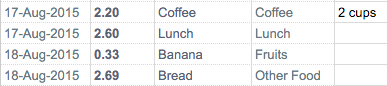
\includegraphics[width=\linewidth]{fig1.png}
	\caption{Snippet of the Dataset.}
	\label{fig1}
\end{wrapfigure}
The dataset lists date of purchase, amount of money spent, item purchased, category and remarks.  In this report we \textbf{focus only on the subset of the data which records the purchase of coffee}. We filtered the dataset and replaced the remarks field with the count of, cups of coffee. Note that:
\begin{itemize}
\item The number of cups for bulk purchases are taken from the of suggested servings on the pack.
\item We had been informed apriori that this consumption pattern is only of a single person.
\end{itemize}

\begin{wrapfigure}{l}{0.7\linewidth}
	\includegraphics[width=\linewidth]{monthly.png}
	\caption{Monthly spend on Coffee}
	\label{fig2}
\end{wrapfigure}
While performing exploratory analysis on the dataset, we observed that the amount of money being spent on coffee has gone down over the months.\ref{fig2}

Although, at first sight this might appear to be a good sign, however this downward trend is because of subject started purchasing coffee in bulk and we \textbf{hypothesise that, bulk purchase of coffee has resulted in its increased consumption}. 

\section*{Our visualization approach}
\textbf{Who is the Target audience of this visualization ?}: This visualization is to help show the trend in coffee consumption to the person whose purchase dataset we are using. 
From the Visualization, the target audience might be interested to know about the number of Cups of Coffee consumed, the corresponding expenditure in Euros and overall trends, if they exist.
To that effect we have aggregated, by month, the Expenditure on Coffee (in Euros) and the number of Cups of coffee purchased (or consumed). This grouping should also average out any daily or weekly fluctuations in the trend.
\section*{Munzner Model}
The following Data \ref{1} and Task \ref{2} abstractions are based on the Munzer model described in the course slides.
\subsection*{Data Abstraction}
\begin{itemize}
	\item Data Type
	\begin{itemize}
		Attribute
		\begin{enumerate}
			\item Date of Purchase 
			\item Cups of Coffee Purchased
			\item Expenditure (Euros)
		\end{enumerate} 
	\end{itemize}
	\item Dataset Type : Table
	\item Dataset Availability : Static
	\item Attributes Types : Quantitative
\end{itemize}
\subsection*{Task Abstraction}
Chained sequence of tasks or {Action, Target} Pairs.
\begin{itemize}
	\item \textbf{PRODUCE : Derive - Distribution}
	\begin{itemize}
			\item Group the Tabular data by Month. 
	\end{itemize}
	\item \textbf{QUERY : Identify - Trends}
	\begin{itemize}
		\item Plot the trend lines
	\end{itemize}
\end{itemize}
\subsection*{Visual Idiom}
A visual idiom is a combination of marks and visual variables which are together called the visual encoding. We describe the visual encoding next.
\subsubsection*{Visual Encoding}
Visual encodings used and their justification.
\begin{itemize}
	\item Marks : Lines
	\begin{itemize}
		\item Bars in the bar plot to encode \textbf{magnitude}
		\item Interpolated lines which aid in the perception of overall trends \ref{6}
	\end{itemize}	
	\item Visual Variables
	\begin{itemize}
		\item Position : \textbf{Horizontal Position of bars}. Aided by the month labels on the x axis, position of the bars can effectively portray ordinal data according to Mackinlay’s ranking of visual variables \ref{3}
		\item Size : \textbf{Length} of bars used to encode \textbf{magnitude} is the best available (Position already used to convey the ordinal month data) visual variable to encode Quantitative Data, according to  \textbf{Mackinlay’s ranking} \ref{3}.
	\end{itemize}
\end{itemize}
\subsubsection*{Description of Visual Idioms used}
\begin{itemize}
	\item We have used \textbf{bar plots} to indicate the \textbf{magnitude} (of Cups of Coffee and Expenditure) as it aids in comparing values. \ref{3}
	\begin{itemize}
		\item Also Bar plots are suitable because, the dataset has 1 key attribute (Date) and 1 quantitative  attribute (either Expense or Cups of Coffee in their respective plots).
	\end{itemize}
	\item We have also used a smoothed (cubic interpolated) \textbf{line plot} as it aids in perceiving \textbf{trends}. \ref{5}
	\begin{itemize}
		\item In this case we used date as the ordered key attribute and the corresponding Expense and Cups of Coffee and the quantitative attribute for the two plots.
	\end{itemize}
\end{itemize}
\section*{Tufte’s Principles}	
\begin{itemize}
	\item We have ensured that the bar plots are proportional to the measured quantities. This follows the principle laid down by Tufte which states that \textit{The representation of numbers, as physically measured on the surface of the graphic itself, should be directly proportional to the numerical quantities represented.}
	\item We use only two visual variables to encode the dimensions of time and magnitude. Conforming with tufte’s principle which states \textit{The number of information-carrying (variable) dimensions depicted should not exceed the number of dimensions in the data.} 
	\item \textbf{Data-ink ratio} is maximized by \textbf{removing the default gray background along with the grids} of the plots (made using ggplot in R). We have \textbf{added light gray horizontal guides} which helps in estimating the quantity represented by the barplots. Also the \textbf{facet bounding boxes are removed}. Although this might cause problems in distinguishing the two faceted plots, we have mitigated this problem by using the Gestalt principle of \textit{connectedness} as described in the next section.
\end{itemize}
\section*{Gestalt Laws} 
\begin{itemize}
	\item \textbf{Continuity} : The overall Trend is better perceived if the trend line is a smooth curve. \ref{7} To that effect, we have smoothed the line plots using cubic interpolation.
	\item \textbf{Closure}: We have made use of facets to draw two graphs with comparable X axis. This is done because Cups of coffee consumed and Spend (in Euros) represent two separate quantities with different units and scales. Visualizing such quantities in the same plot can make the viewer draw false conclusions about the data, this has been discussed extensively in \ref{8} and also in the "Planned Parenthood" example in lecture 2 \ref{facet}.
	\item \textbf{Connectedness} : Horizontal grid lines meet the corresponding facet labels indicating connectedness. This helps in perceiving the two sets of plots as two separate entities as it is a more powerful grouping principle than proximity.\ref{connectedness}
\end{itemize}
\section*{Methods used to analyze the data}
\begin{itemize}
	\item We first filtered the complete set of purchase records to get only the subset of data we were interested in analyzing.
	\item We then \textbf{order the data} by date to ensure that we get the true trend. \textbf{NOTE} : We could get "some" interesting trend and lie with the plots (by not showing the x axis labels) if the data was shown in a random order by date.
	\item We had also \textbf{grouped the data} by month, to get the monthly cumulative expense and cups of coffee consumed. This helped in averaging out small variabilities in the data and made it easier to spot the overall trends.
	\item Finally, instead of drawing a linear trend line we chose to use a \textbf{cubic polynomial} which we thought portrayed the overall trend well without being too jagged.
\end{itemize}
We mainly used the software environment \textbf{R} and its packages \textbf{lubridate} for date transformations, \textbf{sqldf} for data "juggling" and \textbf{ggplot2} for plotting and plot "touch ups", to increase the data-ink ratio.
\end{multicols}
\hrule
\begin{figure*}[h]
	\centering
	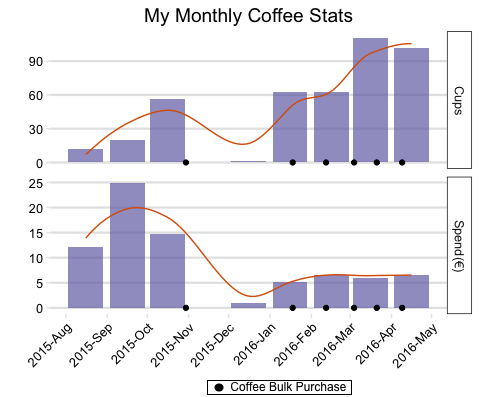
\includegraphics[scale=0.8]{FinalVis-2.png}
	\caption{Note that the consumption is indicative only, if the coffee was purchased on the last day of the month, it would be consumed on the next month. However, it is grouped in the same month in the visualization. That explains why the number of cups don't increase in \textbf{November} after a bulk purchase in October.
	}
	\label{fig}
\end{figure*}
\hrule
\pagebreak
\begin{multicols}{2}
\section*{Chosen Visualization Technique and Rationale}
In this visualization, We have the challenge of visualizing two quantities (Monthly Expense and Cups of Coffee) with different units and scales. It is a known problem \ref{8} that having two scales on the vertical axis leaves scope for manipulative visualizations. Which we have also previously discussed in the section on \textit{Closure} above. 
We could have transformed the data to show only percentage change in the quantities as was done in \ref{Heer} for the stock data for use in Index Charts. However in doing so, the plot would mislead the viewer into thinking the coffee consumption has gone down because, once the number of cups of coffee stays high but relatively constant the percent change would go down. To avoid the above caveat we make use of Facets to show the two quantities in separate graphs. \textbf{Facets} \ref{facetslide}, as also discussed in the "How" to visualize section of \textbf{Munzner's Model},  allow us to juxtapose two graphs such that they have the same Horizontal axis which aids in making meaningful comparisons.
Our choice of colors for the bars and line plot is from a color blind and print friendly color palette  as suggested by the ColorBrewer2.org web-application.
\section*{Results}
After analyzing the data and visualizing it \ref{fig}, we observe that since the bulk purchase (lower coffee spends) have become more frequent, the consumption has risen steadily and shows a positive trend.
\section*{Discussion on Hypothesis after the results: }
The graph quite strongly suggests that bulk purchase (Less monthly expenditure) of coffee has resulted in increased consumption. So we \textbf{can confirm our Hypothesis that the, bulk purchase of coffee has resulted in its increased consumption, based on the above visualization}. Given that the dataset records consumption pattern of only the subject. However it would advisable to run this experiment for a few more months and visualize the trends, to be certain this upward trend wasn't just a coincidence.\\
\vfill
\section*{References}
\begin{enumerate}
	\item Lecture 7 slide 44 - T-61-5010 - Visualization analysis and design  \label{1}
	\item Lecture 7 slide 52 - T-61-5010 - Visualization analysis and design \label{2}
	\item Lecture 7 slide 76 - T-61-5010 -  Visualization analysis and design \label{3}
	\item Lecture 7 slide 79 - T-61-5010 -  Visualization analysis and design \label{5}
	\item Lecture 7 slide 81 - T-61-5010 -  Visualization analysis and design \label{facetslide}
	\item Visualization Analysis and Design Page - (Munzner 2015) page 157 \label{6}
	\item Lecture 6 slide 63 - Human perception part3 \label{7}
	\item Lecture 6 slide 58 - Human perception part3 \label{connectedness}
	\item Lecture 2 T-61-5010 Visualization analysis and design Slide titled "Planned parenthood" \label{facet}
	\item \href{http://www.perceptualedge.com/articles/visual_business_intelligence/dual-scaled_axes.pdf}{Stephen Few (2008) "Dual-Scaled Axes in Graphs
		Are They Ever the Best Solution?"} \label{8}
	\item Jeffrey Heer, Michael Bostock, and Vadim Ogievetsky (2010). "A Tour Through the Visualization Zoo." Communications of the ACM 53(6) : 59-67 \label{Heer}
\end{enumerate}
\end{multicols}
\end{document}
